%\begin{figure}[h]
%    \centering
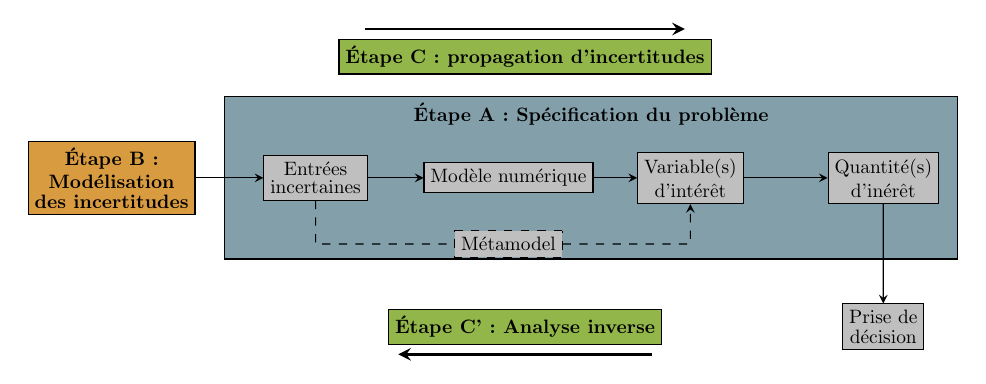
\begin{tikzpicture}[scale=0.7, every node/.style={transform shape}]
    \node[rectangle,draw,fill=YellowOrange!70!gray] (a) at (-9,0) {\shortstack{\textbf{\'Etape B :} \\ \textbf{Modélisation} \\ \textbf{des incertitudes}}};
\node[rectangle,draw,fill=YellowGreen!70!gray] (f) at (-1.5,2.2) {
\textbf{\'Etape C : propagation d'incertitudes}};
\node[rectangle,draw,fill=YellowGreen!70!gray] (g) at (-1.5,-2.7) {\shortstack{
\textbf{\'Etape C' : Analyse inverse}}};
\node[rectangle,draw,minimum width=13.3cm,fill=SkyBlue!40!gray] (h) at (-0.3,0) {\shortstack{\textbf{\'Etape A : Spécification du problème} \\ \phantom{a} \\ \phantom{a} \\ \phantom{a} \\ \phantom{a} \\ \phantom{a} \\ \phantom{a} \\ \phantom{a} \\ \phantom{a} \\ \phantom{a} }};
\node[rectangle,draw,fill=lightgray] (b) at (-5.3,0) {\shortstack{
Entrées\\ incertaines}};
\node[rectangle,draw,fill=lightgray] (c) at (-1.8,0) {\shortstack{
    Modèle numérique}};
\node[rectangle,draw,fill=lightgray] (d) at (1.5,0) {\shortstack{
Variable(s) \\ d'intérêt}};
\node[rectangle,draw,fill=lightgray] (e) at (5,0) {\shortstack{
Quantité(s) \\ d'inérêt}};
\node[rectangle,draw,fill=lightgray, dashed] (i) at (-1.8,-1.2) {Métamodel};
\node[rectangle,draw,fill=lightgray] (j) at (5,-2.7) {\shortstack{Prise de \\ décision}};
\draw[-stealth, black, line width=1pt] (-4.4,2.7) -- (1.4,2.7);
\draw[-stealth, black, line width=1pt] (0.8,-3.2) -- (-3.8,-3.2);
\draw[-stealth, black] (a) -- (b);
\draw[-stealth, black] (b) -- (c);
\draw[-stealth, black] (c) -- (d);
\draw[-stealth, black] (d) -- (e);
\draw[-stealth, black, dashed] (b) -- (-5.3,-1.2) -- (i) -- (1.5,-1.2) -- (d);
 \draw[-stealth, black] (e) -- (j);

\end{tikzpicture}
%    \caption{General uncertainty quantification and propagation framework}
%    \label{Fig:UQ}
%\end{figure}